\documentclass[oneside, a4paper, 11pt]{report}

\usepackage{ngerman}
\usepackage{graphicx}
\usepackage{xcolor}
\usepackage[T1]{fontenc}
\usepackage[latin1]{inputenc}
\usepackage{lmodern}
\usepackage{geometry}
\usepackage[numbers]{natbib}
\usepackage[pagestyles]{titlesec}
\usepackage{titletoc}
\usepackage{microtype}
\usepackage{booktabs}
\usepackage{caption}
\usepackage{subcaption}
\usepackage{setspace}
\usepackage{calc}
\usepackage[colorlinks]{hyperref}
\usepackage{amsmath,amsfonts,amssymb,amsthm}
\usepackage{mathtools}
\usepackage[version=3]{mhchem}
\usepackage{wrapfig}
\usepackage{tikz}
\usepackage{cancel}
\usepackage{algorithm}
\usepackage{algpseudocode}
\usepackage{wasysym}
\usepackage{array}
\usepackage{listings}

\renewcommand\abstractname{Vorwort}

% Layout der "Uberschriften
\titleformat{\chapter}[hang]
{\fontfamily{pag}\Large\bfseries}{\thechapter}{1.5cm-\widthof{\thechapter}}{\large}
\titleformat{\section}
{\fontfamily{pag}\normalsize\bfseries}{\thesection}{1.5cm-\widthof{\thesection}}{\normalsize}
\titleformat{\subsection}
{\fontfamily{pag}\normalsize\bfseries}{\thesubsection}{1.5cm-\widthof{\thesubsection}}{\normalsize} 


\newpagestyle{mystyle}
{
	\headrule
	\sethead{\thechapter. \chaptertitle}{}{\thepage}
	%
	\footrule
	\setfoot{\textnormal{Datenbank}}\raggedleft{\textnormal{Jascha Petter}}
} 
\pagestyle{mystyle}
\parindent0pt
\onehalfspacing
\geometry{outer=20mm,  inner=25mm,  top=20mm,  bottom=30mm}
%
\author{Jascha Petter}
%
\begin{document}
	\begin{titlepage}
		\begin{center}
			
\includegraphics[width=0.4\linewidth]{img/image2.jpg}\\
			\vspace*{3.5cm}
			\Huge{\bf Quadrocopter Raspberry Pi 2016\bigskip\bigskip\\}
			\LARGE{Datenbank mit PythonMySQL\bigskip\bigskip\\}
			\large{Universit"at T"ubingen\vfill}
		\end{center}
		%
		\vspace*{1cm}
		\begin{minipage}{\widthof{Jascha Petter}}
			\begin{flushleft}
				Author:\\
				Jascha Petter
			\end{flushleft}
		\end{minipage}
		\hfill
		\begin{minipage}{\widthof{\today}}
			\begin{flushright}
				Dienstag 20.08.16
			\end{flushright}
		\end{minipage}
	\end{titlepage}
	\begin{abstract}	
		Als Student der Universit"at T"ubingen, in einem der Informatikstudieng"ange, ist die Teilnahme an einem Programmierprojekt vorgesehen. Aus den vielen angebotenen Projekten habe ich mich f"ur das Projekt \glqq{}PiSense mit Quadrocopter\grqq{} entschieden. In diesem Projekt waren die Anpassung der Low Level Treiber, das Darstellen der Sensordaten in einer GUI, eine App zum steuern der Motoren des Quadrocopters, sowie die gemessen Daten in einer Datenbank abzulegen als Ziele gegeben. Die folgende Dokumentation soll das erstellen und Verwalten einer Datenbank, sowie das Empfangen der Daten per UPD beschreiben. 
	\end{abstract}
	%Inhalts- und Abbildungsverzeichnis
	\newpage
	\pagenumbering{Roman}
	\begingroup
	\let\clearpage\relax
	\tableofcontents
	\listoffigures
	\endgroup
	\newpage
	\pagenumbering{arabic}
	%
	\chapter{Einrichtung}
		\section{MySQL}
			\begin{enumerate}
				\item[] 
					Um auf Ihrem System einen MySQL Server laufen zu lassen, ben"otigen Sie den \glqq{}MySQL Community Server\grqq{}.
				\item 
					Laden Sie sich hierzu den MySQL Community Server von der MySQL Homepage herunter.
						\begin{center}
							\url{http://dev.mysql.com/downloads/mysql/}\footnote{stand 20.09.2016}
						\end{center}
					W"ahlen Sie dort die dementsprechende Version f"ur Ihr System. Sie m"ussen sich f"ur den Download nicht anmelden, oder ein Konto erstellen. Klicken Sie einfach auf \glqq{}No thanks, just start my download\grqq{}. 
				\item
					Nach der Installation wir Ihnen das Passwort f"ur den Root User angezeigt.
					\begin{figure}[h!]
						\centering
						\includegraphics[width=0.4\linewidth]{img/rootPW.png}
						\caption{Passwort Alert \label{pw_alrt}}
					\end{figure}\\
					Notieren Sie sich dieses, da es sp"ater noch gebraucht wird!
				\item 
					"Offen sie nun Ihren Terminal und geben folgende Befehle ein, um ein neues Passwort zu vergeben:
					\begin{verbatim}
						$ cd /usr/local/mysql/bin
						$ ./mysqladmin -u root -p password '<password>'
					\end{verbatim}
					Sie werden nun aufgefordert Ihr Root-Passwort, welches Sie vorhin notiert haben, einzugeben.
					\begin{verbatim}
						$ exit
					\end{verbatim}
					Um zur"uckzukehren
				\newpage
				\item
					Nun erstellen wir einen neuen Benutzer und geben diesem die notwendigen Rechte.
					\begin{verbatim}
					$ ./mysql -u root -p
					mysql > CREATE USER 'PiSense'@'%' IDENTIFIED BY 'somePW';
					mysql > GRANT ALL PRIVILEGES ON *.* TO 'PiSense'@'%';
					\end{verbatim}
					Dies ist nun der neue Benutzer, mit dem gearbeitet wird.
				\item
					Nun muss noch der MySQL-Server gestartet werden. Dies ist wie folgt m"oglich.
					\begin{verbatim}
						$ cd /usr/local/mysql/support-files/
						$ sudo ./mysql.server  start
					\end{verbatim}
			\end{enumerate}
		\section{Datenbank}
			\begin{enumerate}
				\item[]
					Da wir nun einen Benutzer zum arbeiten habe, fehlt nur noch die Datenbank und eine Tabelle. 
				\item 
					Zu erst muss ein neues Schema erstellt werden:
					\begin{verbatim}
						$ cd /usr/local/mysql/bin
						$ ./mysql -u PiSense -p
						mysql > CREATE DATABASE `SenseData` COLLATE 'latin1_swedish_ci';
					\end{verbatim}
				\item
					Nun k"onnen Sie eine Tabelle anlegen:
					\begin{verbatim}
						mysql > CREATE TABLE `SenseData`.`DATA` (
						`PITIME` timestamp(2) PRIMARY KEY NOT NULL,
						`ACC_X` double NOT NULL,
						`ACC_Y` double NOT NULL,
						`ACC_Z` double NOT NULL,
						`MAG_X` double NOT NULL,
						`MAG_Y` double NOT NULL,
						`MAG_Z` double NOT NULL,
						`G_ROLL` double NOT NULL,
						`G_PITCH` double NOT NULL,
						`G_YAW` double NOT NULL,
						`TEMP` double NOT NULL,
						`PRESS` double NOT NULL,
						`M1` double NOT NULL,
						`M2` double NOT NULL,
						`M3` double NOT NULL,
						`M4` double NOT NULL
						) ENGINE='InnoDB' COLLATE 'latin1_swedish_ci';
					\end{verbatim}
					Zu den jeweiligen Eintr"agen sp"ater mehr.
			\end{enumerate}
			Jetzt ist die Datenbank vollst"andig erstellt und kann mit Daten gef"ullt werden.
		\newpage
		\section{Python}
			\begin{enumerate}
				\item[] 
					Um sp"ater Daten empfangen zu k"onne und diese in der Datenbank abzulegen ben"otigen Sie Python. Da es sich um eine Skriptsprache handelt, ist eine IDE nicht vonn"oten. Sie k"onnen in Ihrem lieblings Editor ein Skript schreiben. In meinem Fall habe ich mich f"ur Atom entschieden.
				\item
					Laden Sie sich hierzu Python 2.7 von der Python Homepage herunter.
					\begin{center}
						\url{https://www.python.org/downloads/}\footnote{stand 20.09.2016}
					\end{center}
					Nach der Installation, k"onnen Sie "uberpr"ufen ob es sich um die richtige Version handelt mit:
					\begin{verbatim}
						$ python --version
					\end{verbatim}
				\item
					Damit Sie MySQL unter Python verwenden k"onnen, ben"otigen Sie noch MySQL-Python.
					\begin{center}
						\url{https://pypi.python.org/pypi/MySQL-python/}\footnote{stand 20.09.2016}
					\end{center}
			\end{enumerate}
			Nun ist alles komplett und Sie k"onnen beginnen.
	\chapter{Anwendung}
		Aufgabe des Python Skriptes ist es die Daten, welche vom Quadrocopter gemessen und per UDP versendet werden, entgegenzunehmen und in einer Datenbank abzulegen. Hierbei stellt das Skript eine Verbindung zu der Datenbank her und legt dort per INSERTs die empfangenen Daten ab.
		\section{Struktur der Datenbank}
			\begin{figure}[h!]
				\centering
				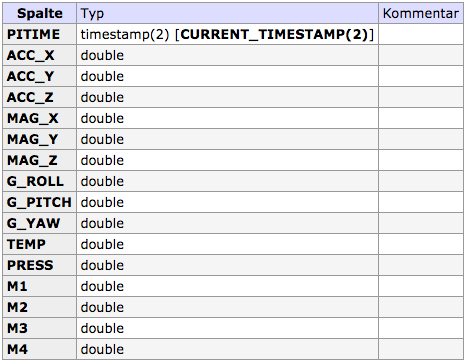
\includegraphics[width=0.4\linewidth]{img/tblstr.png}
				\caption{Struktur der Datenbank \label{db_str}}
			\end{figure}
			\begin{itemize}
				\item \underline{\textbf{PITIME}}\\
					PITIME ist die Zeit, welche momentan auf dem Pi herscht. Sie wurde als Primary Key gew"ahlt, da es zu jeder Zeit nur einen Messwert geben kann. Angegeben wird sie als Timestamp \\
					(YYYY-MM-DD HH:MM:SS:MS) mit einen Genauigkeit von 10ms.
				\item ACC\_X/Y/Z\\
					Es werden alle drei Beschleunigungsachsen gespeichert, das Vorzeichen stellt hierbei die Richtung dar. 
				\item MAG\_X/Y/Z\\
					F"ur das Magnetfeld werden ebenfalls 3 Datens"azte abgelegt. 
				\item TEMP/PRESS\\
					Temperatur und der Luftdruck. 
				\item M1/2/3/4\\
					F"ur die jeweiligen Motoren werden vier Datens"atze abgelegt, da diese sich unabh"anging von einander drehen k"onnen.
			\end{itemize}
		\newpage
		\section{Auszug aus der Datenbank}
			Hier ist ein beispielhafter Auszug der Datenbank zu sehen, er zeigt einen Ausschnitt aus der Demo.
			\begin{figure}[h!]
				\centering
				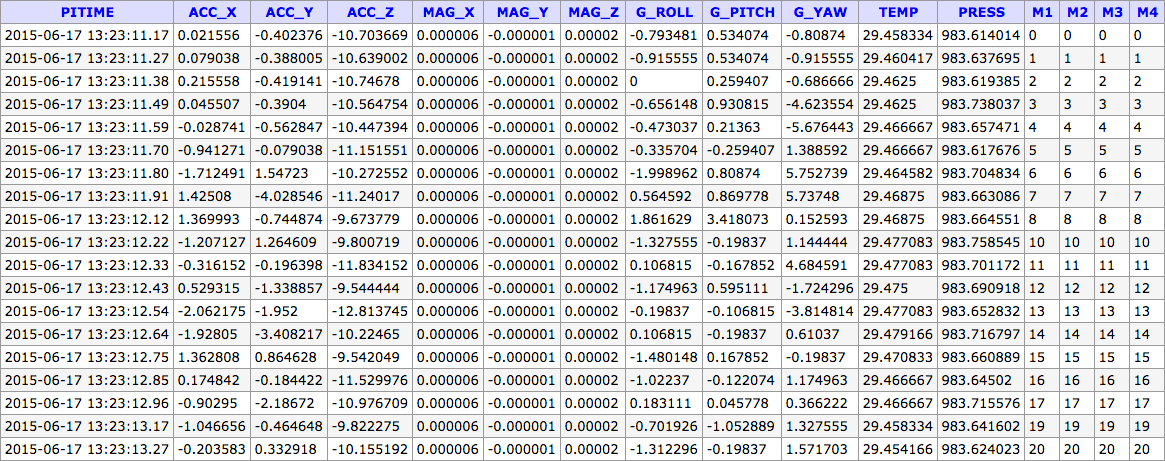
\includegraphics[width=0.9\linewidth]{img/bsptbl.png}
				\caption{Daten der Demo\label{demo_data}}
			\end{figure} 
		\section{Python}
			\subsection{Verbindung zur Datenbank}
				Um auf die vorhin erstelle Datenbank zuzugreifen, muss eine Verbindung hergestellt werden. Hierzu wird der neue Benutzer PiSense ben"otigt, nat"urlich k"onnten man auch Root benutzen das ist aber nicht Sinn der Sache.
				\begin{figure}[h!]
					\centering
					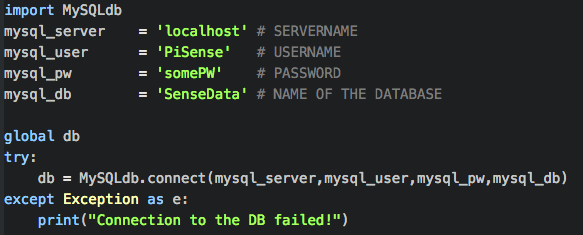
\includegraphics[width=0.65\linewidth]{img/dbc.png}
					\caption{Connector\label{dbc}}
				\end{figure}
			\newpage
			\subsection{UDP Socket}
				Damit das Skipt eine Message vom Quadrocopter empfangen kann, muss ein UDP Socket auf einem bestimmten Port Lauschen. Python stellt uns hierbei einen Receive-Funktion zur verf"ugung. Es muss nur die IP und der Port and einen Socket gebindet werden. 
				\begin{figure}[h!]
					\centering
					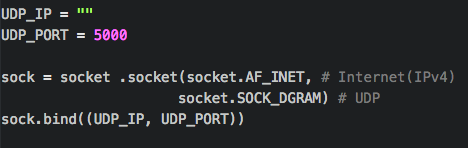
\includegraphics[width=0.65\linewidth]{img/udpsock.png}
					\caption{UDP Socket\label{UDPS}}
				\end{figure}\\
				In diesem Fall lauschen wir auf dem Port 5000, benutzen IPv4 und nat"urlich UDP.
			\subsection{Empfangen und aufteilen der Daten}
				\begin{figure}[h!]
					\centering
					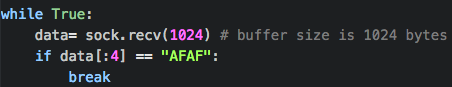
\includegraphics[width=0.65\linewidth]{img/whilerec.png}
					\caption{Empfange der Message\label{recv}}
				\end{figure}
				Es wird so lange gewartet bis eine Message ankommt, falls diese der String "AFAF" ist, wird das Skript beendet. Da die Daten in einem einzigen String ankommen, m"ussen sie herausgefiltert werden. Um dies zu erreichen wird der String bei jedem Zeilenumbruch getrennt. Nun m"ussen noch die Bezeichner \textit{abgeschnitten} werden. Auch hier liefert uns Python einen L"osung mit. Es werden die vier ersten Zeichen verworfen.
				\begin{figure}[h!]
					\centering
					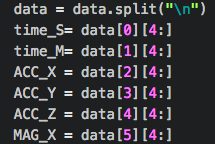
\includegraphics[width=0.3\linewidth]{img/trenn.png}
					\caption{Trennen der Daten\label{trenn_D}}
				\end{figure}
			\newpage
			\subsection{Ablegen der Daten}
				Damit die empfangenen Date jetzt nicht verloren gehen, werden sie in die Datenbank geschrieben. Dies erfolgt "uber einen INSERT. Hierbei werden die Daten in ihre jeweiligen Spalten der Tabelle gespeichert. Am ende muss das Query noch commited werden, an die Datenbank.
				\begin{figure}[h!]
					\centering
					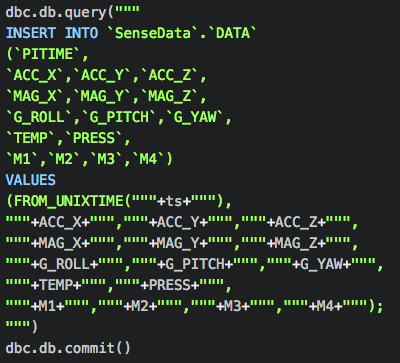
\includegraphics[width=0.5\linewidth]{img/query.png}
					\caption{Query\label{qry}}
				\end{figure}\\	
				Um sicherzustellen, dass das Skript funktioniert kann mit dem \textit{udpSend.py} Skipt ein Senden des Quadrocopters simuliert werden. Jedoch handelt es sich hierbei nur um Zufallswerte. 
			\subsection{Ausf"uhren des Skriptes}
				Das Pythonscript l"asst sich wie folgt ausf"uhren. Wechseln Sie dazu in das Verzeichnis wo die udpReceive.py  zu finden ist.
				\begin{verbatim}
					$ python udpReceive.py 
				\end{verbatim}
				Falls Sie nun das Skript beenden wollen senden Sie per UDP den String \glqq{}AFAF\grqq{}.
				\begin{verbatim}
					$ echo "AFAF" | nc -4u localhost 5000
				\end{verbatim}
		\section{Verwalten der Datenbank}
			\subsection{Adminer einrichten}
				\begin{enumerate}	
					\item[]
						Adminer wurde zum verwalten der Datenbank verwendet.
					\item
						Um mit Adminer zu arbeiten laden Sie dieses von der Adminer Homepage herunter.
						\begin{center}
							\url{https://www.adminer.org/#download}\footnote{stand 20.09.2016}
						\end{center}
					\item 
						Damit Sie Adminer starten k"onne m"ussen Sie die \textit{adminer-4.2.5.php} Datei in ihr Apache verzeichnis verschieben.
						\begin{verbatim}
							$ cd /Library/WebServer/Documents/
						\end{verbatim}
					\item 
						Jetzt m"ussen Sie Apache nur noch f"ur php konfigurieren.\\
						Erstellen sie ein Backoup Ihrer alten Konfiguration.
						\begin{verbatim}
							$ cd /etc/apache2/
							$ cp httpd.conf httpd.conf.bak
						\end{verbatim}
						Nun editieren sie die httpd.conf Datei 
						\begin{verbatim}
							$ vi httpd.conf
						\end{verbatim}
						und kommentieren folgende Zeile wieder ein (die \# enfernen).\\
						\textit{LoadModule php5\_module libexec/apache2/libphp5.so}
					\item 
						Nun muss der Apache nur noch neugestartet werden.
						\begin{verbatim}
							$ sudo apachectl restart	
						\end{verbatim}
				\end{enumerate}
			\subsection{Adminer bedienen}
				\begin{enumerate}
					\item
						Navigieren sie Ihren Browser zu:
						\begin{center}
							\url{localhost/adminer-4.2.5.php}
						\end{center}
					\item 
						Melden Sie sich mit dem Benutzer f"ur die Datenbank an:
						\begin{figure}[h!]
							\centering
							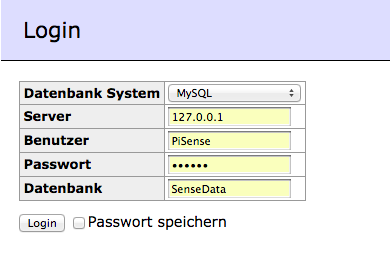
\includegraphics[width=0.55\linewidth]{img/login.png}
							\caption{Anmelden in Adminer\label{login}}
						\end{figure}
					\newpage
					\item
						"Uber das linke Men"u k"onne Sie die Datenbank Verwalten.
						\begin{figure}[h!]
							\centering
							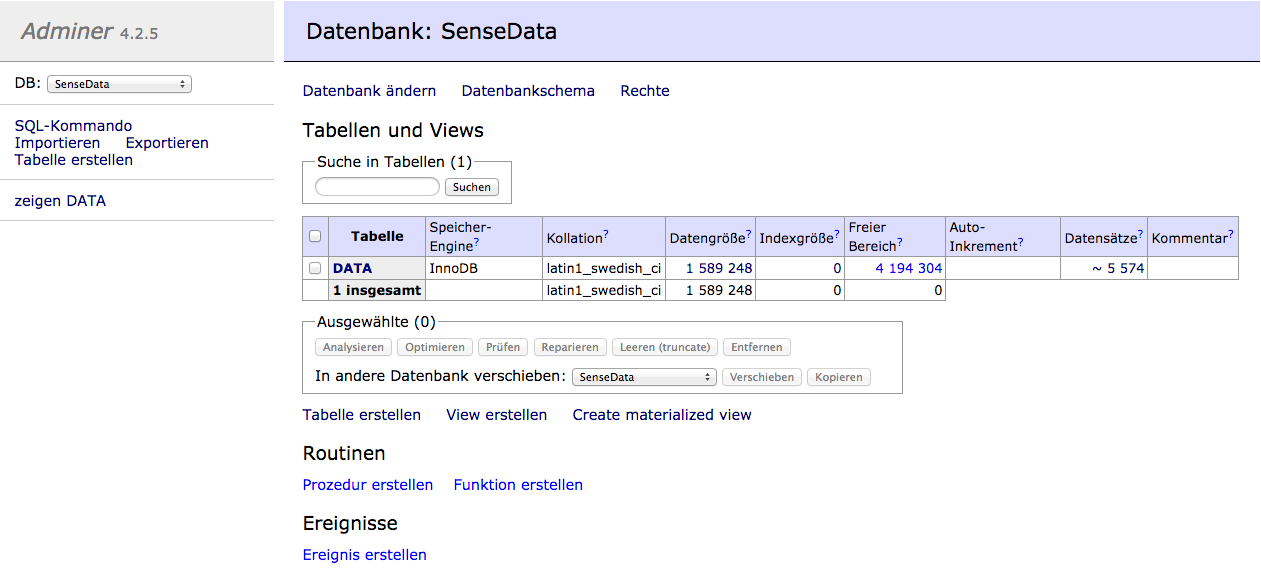
\includegraphics[width=0.9\linewidth]{img/adminer.png}
							\caption{Adminer "Ubersicht\label{ubers}}
						\end{figure}
					\item
						Unter SQL-Kommando k"onnen Sie eingene SQL Anfragen an die Datenbank stellen.
						\begin{figure}[h!]
							\centering
							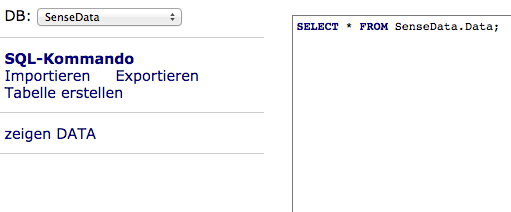
\includegraphics[width=0.55\linewidth]{img/sql.png}
							\caption{SQL-Kommando\label{sql}}
						\end{figure}
					\item 
						Die Importfunktion erm"oglicht es Ihnen einen Dump der Datenbank zu Imporieren. W"ahlen sie dazu einfach eine \textit{sql} Datei aus und klicken auf ausf"uhren.
						\begin{figure}[h!]
							\centering
							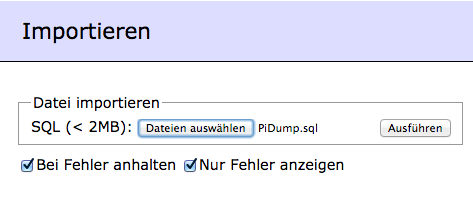
\includegraphics[width=0.55\linewidth]{img/import.png}
							\caption{Importieren einer Tabelle\label{import}}
						\end{figure}
				\end{enumerate}
	\newpage
	\chapter{Zuk"unftige Arbeit}
		\begin{itemize}
			\item Enwiklung einer GUI\\
				Eine GUI, damit die gesammten Skripte nicht mehr von Hand gestartet werden m"ussen.
			\item Verwaltung der Datenbank "uber die Gui\\
				Verwaltungsm"oglichkeit ohne eine externe Software benutzen zu m"ussen, sondern direkt in der GUI.
			\item Erweitern der Datenbank\\
				Die von der Datenbank erfassten Messwerte um weiter erg"anzen, z.B. durch Berechnung aus den aktuellen.
		\end{itemize}
\end{document}
